\chapter{Background}
  The term `Internet of Things' captures the essence of the vision well; the vision of a world where everyday, physical objects are gateways to web-based services. These so-called `smart objects' comprise of sensors to perceive their environment or context, as well as a notion of interconnectivity with other objects or services. Connected objects or services may react to collected data to trigger actions, and these actions may be digital or physical. The Internet of Things could be summarised as data collection, aggregation and reaction in the physical domain.

  The boundaries between IoT and other trends help to define its place in computing. For instance the research area of Wireless Sensor Networks (WSN) carries similarities in hardware requirements and challenges. In particular, WSN also comprise of connected sensors and actuators \citep{Mottola:2011}. WSNs differ from IoT because of the scope of connectivity---they are limited to specific applications and area coverage, such as a production line or a single building. In comparison, IoT applications have a global scope which encourages co-operation between devices, networks and services. Wireless Sensor Networks can, however, form one aspect of an IoT application.

  The research area of `Wearables' also overlaps with IoT. Wearables are smart devices designed to be worn or embedded within the body. They combine sensors with some form of connectivity, typically integrating with a smartphone \citep{6844949}. Consumer Wearables products are already on the shelves, such as Fitbit---a wrist-worn personal health tracker. The Fitbit wristband connects to a smartphone with Bluetooth Low Energy (BLE) and this smartphone then provides global connectivity through its wireless connection. Users can sign-in to a web-based dashboard which will collate and organise personal data. In this scenario, Wearables are collecting, aggregating and reacting to data in the physical domain. Wearables could therefore be described as a subset of IoT (as shown by Figure \ref{iotRelationship}) because they are an application in a specific domain.

  IoT can also take advantage of research conducted for the `Big Data' trend. Over the past three decades, scalable and distributed data management have been a focus for the database research community \citep{Agrawal}. This research originally focused on traditional enterprise applications, but it has expanded to include the Cloud Computing paradigm across two classes of systems: update-heavy applications and ad-hoc analytics \& decision support. IoT is expected to generate large volumes of data and so by leveraging Big Data analytical processes, valuable information can be deduced. For example, Fitbit's web-based dashboard could use Big Data analytics to analyse personal health statistics and to find data trends. 

  IoT also goes some way to realise the Ubiquitous Computing concept. Ubiquitous Computing (also known as pervasive computing) envisages a world where users are surrounded by connected techonology---technology in our homes, workplaces and recreational activities. In his seminal article, \cite{Weiser:1999} notes that ``specialized elements of hardware and software, connected by wires, radio waves and infrared, will be so ubiquitous that no one will notice their presence''. \citet{Lyytinen:2002} take this further and suggest that we will not only be surrounded by technology, but it will be embedded in our social and physical interactions. Research areas such as this not only contribute to the IoT concept but also benefit from its research endeavours.

  \begin{figure}
    \centering
      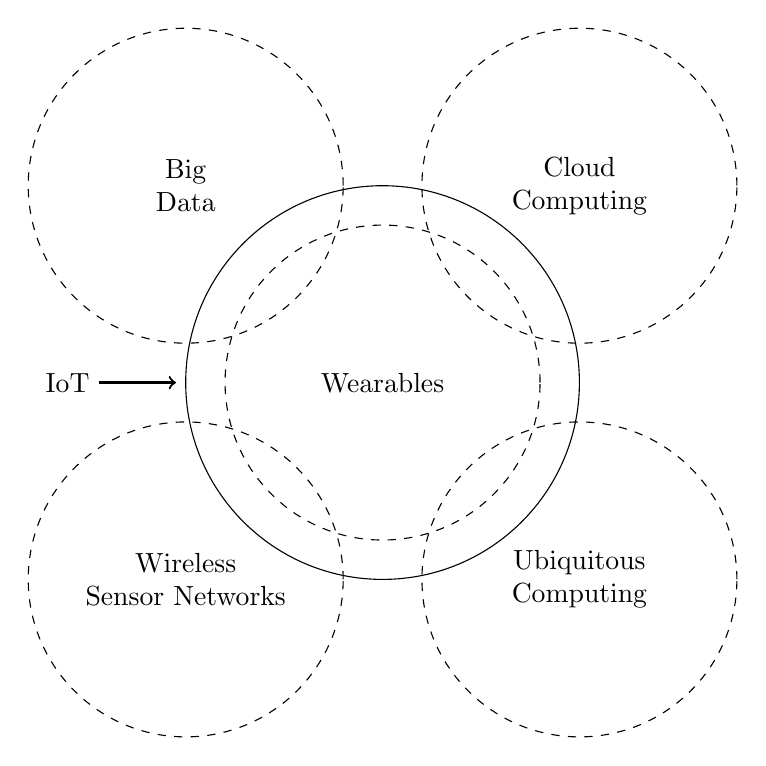
\begin{tikzpicture}
        \node (IoT) at (-2.5,0) {};
        \node at (-4,0) {IoT} edge[->,thick,out=0,in=180] (IoT);
        \draw (0,0) circle [radius=2.5];

        \node[align=center] at (0,0) {Wearables};
        \draw [dashed] (0,0) circle [radius=2];

        \node[align=center] at (-2.5,2.5) {Big\\Data};
        \draw [dashed] (-2.5,2.5) circle [radius=2];

        \node[align=center] at (2.5,2.5) {Cloud\\Computing};
        \draw [dashed] (2.5,2.5) circle [radius=2];

        \node[align=center] at (-2.5,-2.5) {Wireless\\Sensor Networks};
        \draw [dashed] (-2.5,-2.5) circle [radius=2];

        \node[align=center] at (2.5,-2.5) {Ubiquitous\\Computing};
        \draw [dashed] (2.5,-2.5) circle [radius=2];
      \end{tikzpicture}
    \caption{The boundary between IoT and other trends in computing}\label{iotRelationship}
  \end{figure}

  \section{Opportunities}
    Why should we develop IoT solutions? Would our society actually benefit from them? These are the questions posed by stakeholders of all backgrounds. Pilot projects as well as industrial and academic research have shown that there are wide-reaching opportunities to be grasped. Until recently, these opportunities were achievable only in theory or laboratory scenarios, but due to performance improvements and cost reductions in the supporting technology, IoT is very much a reality.

    \citet{fromIoC} describe a number of opportunities created by the evolving technical capabilities of IoT systems. Since much of the value of IoT is derived from the communication of data, the technologies supporting inter-device communication and cooperation are particularly important. Wireless Personal Area Network (WPAN) technologies such as Wi-Fi, Bluetooth, ZigBee and 6LoWPAN give objects the ability to network with Internet resources or each other. These WPAN technologies also provide device addressability mechanisms which allow objects to be uniquely identified from anywhere in the world, through extensions to protocols like MAC Addressing or IPv6. With this level of global interconnectivity, novel services and products become possible.

    Another main characteristic of IoT is the ability to interact with the physical domain. Digital applications will interact with the physical world in two ways: through the monitoring and sensing of physical properties and through the actuation of the physical world in reaction to data. There are a massive variety of sensors available, even to hobby markets, and can measure any imaginable physical property. The reduced cost and improved support by hardware manufacturers will allow measurements to be collected at a scale and precision not previously possible.

    Since IoT microcontrollers are becoming more powerful, there are opportunities for embedded information processing. Embedded information processing refers to end devices performing some form of data processing or storage before transmitting their data; for example, an end device might analyse its own data and only transmit if a specific threshold is met, rather than relying on Cloud Computing-based processing. This is an active area of research called edge computing (or fog computing) and allows for novel methods of data processing and is another method to optimise bandwidth and power consumption.

    Along with these technical capabilities are big-picture societal and economic opportunities. The European Union is a strong example of an economy which can benefit from IoT uptake. The governmental body of the EU, The European Commission, recognises the potential opportunity: ``One major next step in this development [of the Internet] is to progressively evolve from a network of interconnected computers to a network of interconnected objects, from books to cars, from electrical appliances to food, and thus create an ‘Internet of things’.'' In 2009 the Commission published an action plan for embracing the Internet of Things.

    The action plan \citep{ECIoT:2009} describes how IoT will improve citizen well-being both now and into the future. In the present, citizens will benefit from specific IoT initiatives---for instance, Internet-connected health monitoring systems could alleviate pressure on medical services for the ageing society. Other applications such as connected cars or smart waste management are expected to reduce the EU's carbon footprint and therefore protect resources for future generations.

    The Commission's action plan also describes economic opportunties. IoT has the potential to provide many new income streams to businesses as well as finding other money through efficiency savings. First of all IoT opens up new markets which were previously not feasible nor even considered. These markets may include consumer products or novel service solutions in areas such as home security and monitoring. For organisations with complex supply chains or processes, IoT could help to maximise resources and stock control through large-scale automation and efficient information exchange.

  \section{Challenges}
    It is apparent that IoT is still an evolving area of research with numerous challenges to be addressed. In order for IoT to become a mainstream paradigm, the technologies and ecosystem surrounding them must converge and become more mature. \citet{fromIoC} state that IoT is not the result of a single novel technology but rather several complementary technical developments, so invariably, the challenges span many technical disciplines. 

    A good user experience must be offered by these technologies to encourage adoption. \citet{fromIoC} state that devices ``need to establish connections spontaneously, and organize and configure themselves to suit their particular environment'' which they coin `Arrive and Operate'. The process of connecting a laptop to a home Wi-Fi router is representative of the current experience a user might have. They will turn on the Wireless Network Interface Card via a mouse and a Graphical User Interface and select their wireless network before inputing a password with a keyboard. This experience is far from ideal for constrained devices with a simplistic user interface, or no interface at all. The challenge here is to develop technology which allows consumers to use smart objects with little or no configuration.

    Device discovery and interoperability is required to build an open and extensible Internet of Things. Since the world of things is diverse, each type of device is likely to have different capabilities. \citet{interoperability:2015} state that the heterogeneity of existing platforms is considerable (numerous hardware, technologies, requirements and objectives) and as a result, IoT would benefit from a generic architecture which provides IoT developers with a common toolkit. Research efforts have gone some way to address these challenges, such as the IoT `meta-hub' offered by \citeauthor{interoperability:2015}, which provides a feed of available features for a given service.

    IoT infrastructures must be scalable to handle the large number of connections and volume of data. By all estimates, IoT will have a much larger scope and footprint when compared to the existing Internet of computers. The European Commission puts this figure at 50--70 billion devices (on average, 10 per human). \citet{fromIoC} also note that things will be cooperating mainly within a local environment. This means that IoT devices, software and infrastructure must work equally efficiently in both small- and large-scale environments. This complexity is also reflected with the verocity and variety of data being generated; a challenge currently being addressed with research around Big Data.

    Fault tolerance, power supply and efficient wireless communication are challenges facing hardware manufacturers. There are a number of possible operating enviroments for IoT devices, such as office spaces, homes, public spaces and remote areas, so smart objects might depend on a self-sufficient power source. The industry is therefore challenged to produce long-lasting batteries. As well as improving power supply solutions, the industry should maximise power efficiency in other areas such as existing wireless communication technologies which consume too much overhead and power. 

    Technical challenges will continue to be addressed through academic and industrial research, however IoT will not achieve widespread uptake without social acceptance. This is the risk that the industry is carefully attempting to balance; the social acceptance of IoT products is imperative to their success but consumers and markets could be less accepting if industries try too much too soon. The European Commission's action plan describes practical challenges which need to be addressed.

    Many aspects of digital technology is governed by public bodies and the Commission believes that IoT should not be any different. They note that technology will advance due to a normal cycle of innovation and that ``simply leaving the development of IoT to the private section is not a sensible option in view of the deep societal changes that IoT will bring about.'' The main areas which may need to be governed are identification, information security and ethical \& legal accountability. In terms of device identification, \citet{fromIoC} and \citep{ECIoT:2009} suggest that some form public registry (similar to those governed by the Institute of Electrical and Electronics Engineers) will be necessary. In terms of legal accountability, users may be reluctant to use IoT services unless there are safeguards in place. Without effective governance of these areas, IoT may suffer from stifled innovation; a mistrust with data and jeopardised system integrity.

    Standardisation is a technical consideration but also impacts on the economic potential of IoT. The purpose of a standard is to give different entities and stakeholders a common language to design, build or communicate. The widespread adoption of a standard gives businesses of all sizes the opportunity to develop interoperable solutions. In being interoperable, standards-based solutions will be suitable for a wider market and in turn, this will encourage innovation and improve international competitiveness. If IoT is to maximise economic impact and to benefit from widespread adoption, there must be accepted practices or formal standards in place.

    The greatest challenges to social acceptance are security and data privacy, particularly in the EU where the protection of privacy and personal data are two fundamental rights. The challenge with this, in respect to IoT, is that new methods of collecting and using data will be invented. Does current legislation and safeguards protect the interest of EU citizens adequately? Who will own the data---the user whom it is about or the organisation that captured it? The Commission suggests that in response to this challenge, IoT components should be designed from their inception with a privacy- and security-by-design mindset.

  \section{Use Cases}\label{use-cases}
    Use-cases are a helpful mechanism for demonstrating the IoT concept. It is a difficult concept to explain because there are many cooperating components and ideas and for this reason, research papers exemplify their arguments with practical examples. Although IoT applications could be developed for virtually any industry there are domains where its application is more obvious. Table \ref{iot-overview} presents six such domains for IoT, together with opportunities, challenges and related areas of research.

    `Smart Cities' is a vision which convincingly demonstrates many benefits of IoT. \citet{DfBIS:2013} describes the main issues facing local authorities which includes: piecemeal urban infrastructure, climate change targets, the changing nature of the high street and elderly social care. The economic downturn has also reduced budgets assigned to local authorities by as much as 30\% between 2010 and 2013 making cost efficiencies another issue. By developing or retrofitting urban infrastructure with IoT connectivity, local authorities can monitor services in much finer detail. For instance, Bigbelly Solar is a smart waste and recycling system. The Internet-connected waste bins allow local authorities to monitor their status and to schedule collections when they are full. \citet{fog:2012} also describe a system of smart, connected traffic lights which can control the traffic flow through a whole city, reducing congestion and improving safety.  

    IoT in the utilities sector is one use-case which has started to become realised. The British Government is requiring energy companies to install smart meters for their customers and expect most to have a smart meter installed by 2020 \citep{DoECC:2013}. Smart meters monitor domestic energy usage on a per-site basis and can give real-time information about how much electricity is being used, expressed in pounds and pence. For individual households this has the benefit of enabling homeowners to save money and to reduce emissions. At a national level, smart meters are a step towards reducing energy consumption and meeting climate change goals. This use case is particularly interesting and well documented, so section \ref{case-study} investigates the smart meter concept further. Additionally, smart thermostats like Nest also allow households to minimise their gas consumption and to reduce heating bills. This is achieved through usage optimisation based on occupancy patterns. 

    Logistics is one area which demonstrates the efficiency savings that an IoT application can make. \citet{ECFreight:2007} states that ``Freight Transport Logistics focuses on the planning, organisation, management, control and execution of freight transport operations in the supply chain'' and notes that it is one of the drivers of European competitiveness. To remain competitive, this industry must continue to improve and streamline infrastructure, fleet management and goods tracking. IoT could be used to share content-related data and location information for regulatory or commercial purposes. This is achieved through the use of inexpensive RFID tags (which store specific information about the item) and GPS sensors (which can identify precise locations). This would reduce time spent by workers manually recording goods and it will reduce errors at interchange points. The Commission has coined this the `Internet for Cargo'.

    \begin{table}
      \scriptsize
      \begin{tabularx}{\textwidth}{|X|X|X|X|X|X|}
        \hline
        \multirow{3}{2cm}{\textbf{Overlapping Research}}
          & \multicolumn{2}{|c|}{\textbf{Opportunities}}
          & \multicolumn{2}{|c|}{\textbf{Challenges}}
          & \multirow{3}{2cm}{\textbf{Example \newline Use Cases}} \\ \cline{2-5}
          & \textbf{Economic \newline \& Societal}
          & \textbf{Technical} & \textbf{Economic \newline \& Societal}
          & \textbf{Technical}
          &
        \\ \hline
          Cloud Computing
          & Citizen Well-Being
          & Communication \& Cooperation
          & Governance
          & `Arrive and Operate'
          & Smart Cities
        \\ \hline
        Big Data
          & Economic Prosperity
          & Addressability
          & Standardisation
          & Interoperability
          & Waste Management
        \\ \hline
          Ubiquitous Computing
          & Ageing Society
          & Identification
          & Security & Discovery
          & Smart Traffic Lights
        \\ \hline
          Wireless Sensor Networks
          & New Markets
          & Sensing
          & Data Privacy
          & Software Complexity
          & Utilities
        \\ \hline
          Wearables
          & Business Optimisation
          & Actuation
          & Trust
          & Scalability
          & Smart Meters
        \\ \hline
          Edge Computing
          &
          & Localisation
          &
          & Data Management
          & Logistics
        \\ \hline
          &
          & Embedded Information Processing
          &
          & Fault Tolerance
          &
        \\ \hline
          &
          & User Interfaces
          &
          & Power Supply
          &
        \\ \hline
          &
          &
          &
          & Wireless Communication
          &
        \\ \hline
      \end{tabularx}

      \caption{A summary of the current state of the Internet of Things}\label{iot-overview}
    \end{table}
    
  \section{Existing Platforms}\label{existing-platforms}
    \subsection{Overview}
      Now that a baseline has been established for Internet of Things research, it is possible to investigate specific technologies and architectural decisions. There are already numerous IoT platforms both in service and under active development; in fact, Amazon announced their own platform (Amazon IoT) when writing this very comparison and not long after, Digi refreshed their own platform product, showing just how dynamic this area currently is.

      The aim of an IoT platform and the tools which it provides does differ from vendor to vendor but after comparing some headline features, there are various characteristics common amongst them. The platforms were chosen by sifting through marketing websites online and paper lists, like that by \citet{contemporaryIOT:2015}, before selecting a representative sample of organisations. The platform offerings were analysed and compared against five common characteristics: hosting model, source availability model, connectivity, bidirectional communication support and trigger support.

    \subsection{Hosting}
      The hosting model offered by an organisation defines which stakeholder is responsible for maintaining the IoT application and its supporting infrastructure---the platform provider or the customer. This is notable differentiator between platforms and can be indicative of the platform vendor's business objectives (which also relates to the Source Availability Model, coming up next). There are generally two variations in hosting models: Platform as as Service (PaaS) or self-hosting.

      \subsubsection{Platform as a Service}
        A Platform as a Service (PaaS) is a Cloud Computing concept. It is an abstraction of the complete application technology stack including both hardware and software. An organisation providing a PaaS would be reasonable for the management and maintenance of the hardware such as servers, RAID backing storage and networking appliances like routers or switches. Depending on the software on offer, the vendor would also be responsible for managing and maintaining the server operating system as well as any supporting software packages and applications. Customers are typically provided access to this abstraction through a control panel or an Application Program Interface (API).

        In the context of the Internet of Things, a PaaS would provide various benefits to a customer. Primarily the customer do not need to allocate resources for infrastructure maintenance since the vendor manages this, with the result being more time for the customer to focus on business needs. There is also less investment required on behalf of the customer---PaaS resources can be provisioned when and if they are needed, rather than purchasing hardware upfront. Another benefit is the extra layer of support---system scalability, stability and fault tolerance are the responsibility of the PaaS vendor. One example of a PaaS is \href{https://www.carriots.com/}{Carriots}.

      \subsubsection{Self-hosted}
        An alternative to a Platform as a Service is the self-hosted option. As the name implies, this option makes customers responsible for the maintenance and management the application infrastructure (although software updates may still be provided by the platform vendor). There are technical and legal arguments to support such a business decision.

        The main technical aspect is that of control. With the self-hosted option, the system architecture can be optimised for specific use-cases, such as the global location of servers to reduce application latencies (the time taken for network transmissions between devices and server). This also gives customers direct access to the core software and makes it easier to modify it for their own purposes (if the licence or software allows for that).

        Self-hosting may also be necessary for legal compliance, especially in the realm of data protection. Depending on the country of operation, it may be necessary to retain data within country boundaries and this may not be enforceable with a PaaS. For example, in October 2015 the Court of Justice of the European Union ruled that the Safe Harbour agreement between the EU and United States is invalid \citep{C362/14}. This means that any organisation sharing data under this agreement is now acting unlawfully---a problem which could be avoided if data is managed from within the European Union. One example of a self-hosted platform is \href{http://nitrogen.io/}{Nitrogen.io}.

    \subsection{Source Availability Model}
      The Source Availability Model chosen by a platform developer defines the level of accessibility for their source code. This model comes in two forms---open or closed source---and can be further refined by a software license framework.

      The source code of Open Source Software (OSS) is made publicly available. This could be served as a standard file download or, as is becoming common practice, on a code sharing service such as Github or Bitbucket. OSS will typically be provided under the conditions defined in a license, such as the GPL, MIT or Apache license frameworks. These vary on various points like distribution, modification and notification of copyright \citep{license:2015}.

      Closed Source Software is proprietary source code not made publicly available, although it may be necessary to distribute compiled binaries. This just means that the organisation does not wish to make source code available for modification or knowledge sharing. 

      In conjunction with the hosting model, the source availability is indicative of business objectives. Organisations wishing to commercialise their platform as a product offering will use a Closed Source model to protect their intellectual property. Conversely those organisations where knowledge sharing is an aim, or where the platform is a mechanism to sell other products or services (such as \href{https://data.sparkfun.com/}{Sparkfun} and their electronic hardware) may use an Open Source model.

    \subsection{Connectivity}
      The Internet of Things concept \emph{is} interconnectivity and communication, making device and application connectivity a very important topic. The platforms investigated support a range of connectivity protocols and concepts. These range from widely-accepted HTTP-based APIs to more niche protocols like CoAP and MQTT.

      \subsubsection{HTTP}
        The Hypertext Transfer Protocol (HTTP) underpins the internet. It benefits from widespread support and most notably, is used by web browsers to interface with web servers. RFC 2616 \citep{rfc2616} defines the specification for HTTP version 1.1 and notes:

          \begin{quote}It is a generic, stateless, protocol which can be used for many tasks beyond its use for hypertext, such as name servers and distributed object management systems, through the extension of its request methods, error codes and headers.\end{quote}

        As hinted at by this RFC 2616 quote, three important features of HTTP are request methods, error codes and headers. To generalise the HTTP life cycle, a user agent will send a request to an origin server, the server will process the request and will return a response. The request will use an HTTP \emph{verb} to define the action to take, such as \code{GET} or \code{POST}, and will include headers to specify other parameters. The response has an associated status code, such as \code{200 OK} or \code{404 Not Found}.

        Most of the platforms investigated support HTTP requests through a Representational State Transfer (REST) API. \citet{rest:2000} states that the REST architectural style emphasises scalability, independence of components, minimises latency and maximises security. These characteristics are achieved by applying constraints to the application, such as stateless communication, a uniform component interface and a layered approach to infrastructure technologies. REST methods are based on the HTTP verbs, such as \code{GET}, \code{POST}, \code{PUT} and \code{DELETE}. For IoT application developers, a REST API provides a scalable, uniform and robust interface between devices and the Internet. % JSON & XML

        Software engineers working on specifications for the Internet have foreseen the Internet of Things, even if it was taken in jest. RFC 2324 \citep{rfc2324} is an April Fool's joke and defines the Hyper Text Coffee Pot Control Protocol version 1.0 (HTCPCP/1.0). It specifies methods by which an Internet-connected coffee pot can be controlled, and even adds a new error code: ``Any attempt to brew coffee with a teapot should result in the error code `\code{418 I'm a teapot}'. The resulting entity body MAY be short and stout.''

      \subsubsection{WebSockets}
        The WebSocket Protocol is an independent TCP-based protocol that enables two-way communication. It uses an HTTP request as part of the handshaking process, which is treated as a connection upgrade request. RFC 6455 \citep{rfc6455} states ``The goal of this technology is to provide a mechanism for browser-based applications that need two-way communication with servers that does not rely on opening multiple HTTP connections (e.g., using \code{XMLHttpRequest} or \code{\textless iframe\textgreater}s and long polling).'' This technology plays a vital role in enabling bidirectional communication between web browsers and servers, as will be covered in section \ref{bidirectioncomms}.

        WebSockets use standard HTTP ports for communication by default (port 80 and 443 for unencrypted and encrypted connections respectively). This has the added benefit of being compatible with common network and firewall configurations.

      \subsubsection{MQTT}
        MQ Telemetry Transport (MQTT) is a simple and lightweight messaging protocol. It is based on a publish/subscribe model and is specifically designed for constrained devices and low-bandwidth, high-latency or unreliable networks. In general, MQTT is used in conjunction with a message broker. Clients subscribe to topics on this broker which will then forward any relevant messages. Clients are then free to do whatever they please with these messages \citep{mqtt:2015}.

        MQTT uses TCP/IP to transmit messages and operates on ports 1883 and 8883 for unsecured and secured uses respectively. Since these ports and not common, firewalls will typically block access. For this reason, MQTT can be tunnelled using WebSockets (and means this can be used in the browser, too).

      \subsubsection{CoAP}
        Constrained Application Protocol (CoAP) is another protocol designed with the Internet of Things in mind. \citet{rfc7252} describe CoAP as ``a specialised web transfer protocol for use with constrained nodes and constrained networks.'' Some headline features align with principles used with HTTP, such as utilisation of the REST model. RFC 7252 defines the proposed specification for CoAP. It specifically notes some main features:

        \begin{itemize}
          \item Web protocol fulfilling M2M requirements in constrained environments
          \item UDP [RFC0768] binding with optional reliability supporting unicast and multicast requests
          \item Asynchronous message exchanges
          \item Low header overhead and parsing complexity
          \item URI and Content-type support
          \item Simple proxy and caching capabilities
        \end{itemize}

        CoAP is likened to HTTP throughout the specification however there are some notable differences. HTTP uses the TCP/IP transport protocol whereas CoAP uses UDP, a protocol with significantly less overhead. UDP is not a request/response protocol so to provide a request/response interaction model, CoAP must deal with this through a logic layer.

      \subsubsection{UDP}
        One of the researched platforms also offers the User Datagram Protocol (UDP) as a connectivity option. RFC 768 \citep{rfc768} notes ``this protocol provides a procedure for application programs to send messages to other programs with a minimum of protocol mechanism.'' To achieve `a minimum of protocol mechanism', UDP does not establish a connection with the receiving device, so unlike TCP/IP it is connectionless. The protocol also specifies no mechanism for error correction so if a packet is lost in transit, it is lost forever.

        Since data can be lost, this protocol should only be used in applications which can tolerate data loss. To give a real-world example, a battery-powered hygrometer sensor may be collecting data about the enviromental humidity. If UDP was used as the connectivity protocol, it would allow this sensor to wake up, transmit its reading and then fall back to sleep without being concerned about the packet's progress. If a packet was lost, it would not have business or safety impacts.

    \subsection{Bidirectional Communication} \label{bidirectioncomms}
      One main opportunity of IoT, as described in Section \ref{TechnicalOpportunities}, is to drive actuators in response to data. There are three aspects which define whether unidirectional or bidirectional communication is possible: the connectivity protocol, the software application and the network environment. To illustrate the following points, a hypothetical scenario will be used, where one server and one actuator are connected together through the internet. In this case, unidirection communication means that only the actuator can initiate network requests whereas bidirectional communication allows either the server or actuator to initiate.

      If the actuator is publicly addressable with a dedicated IP address, bidirectional communication is trivial to implement. Supposing that the HTTP protocol is being used for communication, both the actuator and server can initiate requests to each other by using the appropriate IP address. The server may send an HTTP request instructing the actuator to do something, and it obey. In real-world scenarios, there are three factors which make bidirectional communication like this difficult: firewalls, Network Address Translation and IPv6 uptake.

      Firewalls are common-place both in businesses and at home. They are a network security tool and can be either a dedicated hardware unit or software built into other devices, such as a domestic router. Their purpose is to screen both in and outbound connections which may have a malicious or compromising effect on the network integrity. The side effect which this has on IoT systems is that non-common protocols may be blocked, such as MQTT (since it uses ports 1883 and 8883). While devices behind a firewall may be publicly addressable, they may not be reachable, depending on the IoT application.

      While obtaining a public IP address for each IoT device is a worthy aim, it is not achievable in many situations due to Network Address Translation. Network Address Translation (NAT) is a tool used to delay the depletion of IPv4 addresses and is very common with domestic internet connections. RFC 2663 \citep{rfc2663} states ``NAT devices are used to connect an isolated address realm with private unregistered addresses to an external realm with globally unique registered addresses.'' In essence, this allows a number of privately addressed devices to communicate through one public address. In terms of IoT, this means than any devices connected behind NAT will not be publicly addressable---the server could not directly send a request to the actuator.

      Internet Protocol version 6 (IPv6) will solve the issue of IP address depletion. It will offer over 340 undecillion possible addresses, compared to just under 4 billion available from IPv4, and will allow every connected device to have its own IP address for the foreseeable future \citep{ipv6:2008}. With regards to the Internet of Things, this is still not achievable. IPv6 is still not supported by many internet service providers (ISPs) and networks, including that of Robert Gordon University. For the Internet of Things, this means that universally supported IPv6 is still a while off.

      There are some useable techniques to overcome these three issues and to enable (or mimic) bidirectional communication. The first of these solutions is HTTP polling. With standard polling, the actuator would periodically ask the server for updates. If this period was 1 second, the communication may feel like it was real-time and bidirectional. This is however wasteful because not every request will result in an update. A more efficient form of polling is called long polling. The actuator will send a request to the server, but if there are no updates yet, the server will not respond. When the server does have a message to send to the actuator, it will respond and then end the request. This is better, but implementations suffer from the added complexity of managing connections, and it is using the HTTP specification in a way it was not designed.

      A final and more effective solution is to implement communication using WebSockets. As previously described, the WebSocket protocol allows for bidirectional, full duplex communication and it can solve every challenge already addressed. WebSockets use the same communication ports as HTTP (port 80 and 443) by default, meaning that firewalls will allow them. Networks that support web browsing will support WebSockets. Also, the WebSocket connection can be initiated by the client and still allow bidirectional communication. In this case, the actuator can open a WebSocket connection to the server and overcome any Network Address Translation in place because it does not require a public IP address.

    \subsection{Application Triggers}
      One application-level feature common across investigated platforms is some form of event trigger. Where supported, platforms can trigger actions based on the data received from sensors and third-party APIs. Combining examples already mentioned, a hygrometer may send data to an IoT application. An application trigger could be configured to turn on a dehumidifier actuator if the humidity passes a certain threshold. If bidirectional communication is supported, this trigger would react in real-time. Triggers could also be configured to interact with other third-party software APIs.

      \begin{table}
        \scriptsize
        \begin{tabularx}{\textwidth}{|X|X|X|X|X|X|}
          \hline
          \textbf{Service} & \textbf{Hosting} & \textbf{Source} & \textbf{Connectivity} & \textbf{Bidirectional} & \textbf{Triggers} \\ \hline
          Amazon IoT & PaaS & Closed & MQTT, HTTP & Yes & Yes \\ \hline
          Bug Labs Dweet & PaaS & Closed & HTTP & Yes (app) & No \\ \hline
          Carriots & PaaS & Closed & HTTP, MQTT & No & Yes \\ \hline
          Sparkfun & PaaS or self-hosted & Open & HTTP & No & No \\ \hline
          Exosite & PaaS & Closed & CoAP, HTTP, UDP & No & Yes \\ \hline
          Google Brillo & PaaS & Closed & Unknown & Unknown & Unknown \\ \hline
          Digi & PaaS & Closed & HTTP & Yes & Yes \\ \hline
          IFTTT & PaaS & Closed & HTTP & No & Yes \\ \hline
          Newaer & PaaS & Closed & HTTP & No & Yes \\ \hline
          Nimbits & Self-hosted & Open & HTTP & No & Yes \\ \hline
          nitrogen.io & Self-hosted & Open & MQTT, HTTP & Yes & Yes \\ \hline
          ThingSpeak & PaaS or self-hosted & Open & HTTP & No & Yes \\ \hline
        \end{tabularx}

        \caption{Characteristics of existing IoT platforms}\label{platform-characteristics}
      \end{table}
  \section{Sensor Hardware}\label{sensor-hardware}
    \subsection{Overview}
      The Internet of Things is a multidisciplinary area of research and is just as dependant on advancements in electrical and electronics engineering as it is computer science. Since the hardware driving IoT sensor nodes is intertwined with the upper layers of software, it would be appropriate to investigate the current state of this area too. Rather than research the intricacies of how these pieces of hardware work, this paper will investigate existing end device hardware with regards to their implementation in IoT applications, particularly technical capability and energy efficiency.

      With a similar method to Section \ref{existing-platforms}, various makes and models of hardware boards were analysed to find comparable characteristics. The manufacturers chosen---Arduino, Raspberry Pi, Intel and Samsung---represent a cross-section of the field. These manufacturers aim their products at different markets, from the DIY `maker' market of the Arduino to the professional, consumer electronics market of Samsung. This section will compare and contrast hardware models produced by these manufacturers across a range of key areas: processor architecture, memory, input/output options and wireless connectivity. Table \ref{hardware-boards} summarises each model and their specifications.

    \subsection{Processor Architecture}
      Just like any other computer system, the processor is the heart of the hardware board. It is responsible for running the operating system, orchestrating the various system components and for running the user application. The type and specification of the processor defines what can be processed and how quickly, which is ultimately reflected in the responsiveness and capability of the IoT device. Processor throughput is not the only consideration when scoping an IoT device however---energy consumption is also an important factor. The specification of the processor can be categorised into smaller areas: processor type, instruction set, number of bits, clock speed and the number of cores.

      There are two broad types of processor systems, namely microcontrollers and microprocessors. A microcontroller (also known as an embedded controller) is a complete computer in one chip. A single microcontroller chip will typically combine a central processing unit (CPU), small amounts of program memory and Random Access Memory (RAM) and input/output lines \citep{microcontrollers:2011}. In comparison, a microprocessor requires other system components to function, such as external memory, input/output lines and a clock circuit. In this regard, microprocessor hardware cannot be upgraded because it is integrated whereas a microprocessor system can, but they are cheaper to manufacture.

      Processor architecture can also vary between makes and models. \citeauthor{microcontrollers:2011} notes that processors can be classified by the number of bits they process, with 8 bits being the most popular for microcontrollers. Processors with a greater number of bits are more powerful but are also more expensive. The instruction set used also effects the performance of the processor; Reduced Instruction Set Computer (RISC) instructions take only one CPU cycle to complete whereas Complex Instruction Set Computer (CISC) instructions can take multiple cycles.

      Clock speed and the number of cores are two final factors of a processor's performance. The clock speed describes how many cycles the CPU executes in one second and is regulated by a crystal timer or internal digital clock oscillator (DCO) A greater clock frequency means more instructions which can be processed in a time period, and the more powerful the processor. Microcontrollers typically have clock speeds in the tens of Megahertz whereas microprocessors might run at hundreds of Megahertz or a number of Gigahertz. However due to physical limitations of hardware components, there is a practical limit in possible clock speed. In this case more cores are added to the processor allowing it to evaluate multiple instructions concurrently. With regard to power consumption, \citet{wsnpower:2010} state that clock speed is one factor affecting the lifetime of a battery powered device so the CPU should be carefully considered for its application.

    \subsection{Memory}
      In any computer system, different types of memory are used to store program instructions and the temporary data associated with them. While these types of memory can be split into more discrete categories, there are generally two types of memory: non-volatile and volatile. Non-volatile memory, such as Read-Only Memory (ROM) or Programmable Read-Only Memory (PROM), is used to store program instructions and fixed user data. Non-volatile memory is used to store this kind of data because it is not lost when power is disconnected. In comparison, volatile memory loses its contents when power is removed and so it is used for temporary or intermediate data.

      Memory characteristics also contribute to the capabilities and performance of the hardware system. Primarily, the available memory size defines how much data can be stored. The Arduino boards researched have 32KB of program memory available compared to the Gigabytes available on some Samsung Artik boards. This constrains the number of program instructions which can be stored and means the software running on the Samsung Artiks could be much more complex. Memory word length also has implications. The word length is the number of bits which a single unit in memory can store, and is commonly found to be 8, 16, 32 or 64 bits. Larger word lengths can store larger pieces of instructions or data, such as larger numbers. 

    \subsection{Input/Output}
      The Input/Output (I/O) lines of a hardware board are the interface between sensors or actuators and the processor (or beyond). Without this physical connectivity, developers would not be able to capture information about the physical world, stopping the IoT concept in its tracks. This aspect of hardware boards is therefore important to the flexibility and future potential of IoT applications. To ensure compatibility between hardware platforms and external hardware like sensors, various industry standards have been developed.

      Before any I/O standards are discussed though, it is first important to establish the importance of the operating voltage for an individual electronics circuit. The hardware boards analysed operate at various logic voltages; for instance most Arduino boards run at 5V whereas the native voltage of the Intel Edison is 1.8V. The standard logic voltage also effects I/O operation. Digital sensors may have their own, incompatible standard logic voltage---a microcontroller running at 5V would damage a sensor running at 3.3V. If directly interfacing between processors and sensors, a logic level shifter might have to be implemented so careful planning is required. Logic voltage is another aspect which affects the lifetime of a battery-powered node \citep{wsnpower:2010}.

      General Purpose Input Output (GPIO) pins are a blank canvas for engineers and developers. They are digital I/O pins with no default use and as their name suggests, can be configured as input or output. Since they are digital, GPIO pins can only read or write with 2 discrete values, logic high (1) or logic low (0), and these values usually respect the standard system voltage. Depending on the device, a number of GPIO pins might support Pulse Width Modulation (PWM). PWM is a technique for emulating analogue levels by pulsing the digital value at differing frequencies. Using a light bulb as an example, PWM could emulate the effect of dimming the light, like what could be achieved with an analogue potentiometer.

      While GPIO pins allow for basic I/O operations, there is a need for communicating with more complex data. There are various available standards for interfacing between low-level electronics components. The datasheets for the selected model note some common standards, namely: Serial Peripheral Interface (SPI), Universal Asynchronous Receiver/Transmitter (UART), Inter-Integrated Circuit (I\textsuperscript{2}C) and Integrated Interchip Sound (I\textsuperscript{2}S). There are a variety of uses for these standards so this paper will go no further than noting that they exist.

    \subsection{Connectivity}
      Interconnectivity is yet one more important aspect to hardware designed for the Internet of Things. Since IoT devices are becoming increasing mobile and wire-free, connectivity is being discussed almost exclusively in regards to wireless communication protocols and standards. As was discussed in Section \ref{TechnicalOpportunities}, some IoT-specific wireless standards have already been established. Many of these technologies are supported by the various hardware platforms investigated, validating their purpose. The standards supported by these hardware platforms are IEEE 802.11 (Wi-Fi), Bluetooth and IEEE 802.15.4 (Low-Rate Wireless Personal Area Network). 

      Wi-Fi is a technology which has become synonymous with wireless connectivity and the Internet. The IEEE 802.11 standard states that the purpose of Wi-Fi is ``to provide wireless connectivity for fixed, portable, and moving stations within a local area'' where a local area could refer to a home, classroom or office space. Wi-Fi benefits from wide utilisation in all areas and industries so wireless coverage is likely to be in place already. \citet{wifiah:2012} state that the radio frequencies used by Wi-Fi (2.4GHz and 5GHz bands) are becoming crowded and are increasingly resulting in radio interference. This is being addressed in a new standard, IEEE 802.11.ah, which makes use of the 900MHz frequency band. The two main potential advantages of this standard are greater range and less power consumption, which is beneficial to IoT devices. Even with this standard, however, end devices are impeded by the large overhead of upper layer protocols used in conjunction with Wi-Fi.

      The Bluetooth standard has been repurposed as an effective wireless communication protocol for IoT devices. Prior to the introduction of Bluetooth 4.0 in 2010, it was primarily used in multimedia applications such as streaming stereo audio \citep{bluetooth:2014}. With the introduction of Bluetooth 4.0 came new features, namely Bluetooth Low Energy (BLE), which consumes such a small amount of power that a sensor can run from a coin battery for months or years. For an average usage scenario, BLE could be expected to achieve a practical maximum range of 77 meters \citep{linklabs:2015} which makes it ideal for use-cases such as body sensors and intelligent transport systems.

      One final wireless connectivity standard supported by the investigated hardware is IEEE 802.15.4 Low-Rate Wireless Personal Area Networks (WPAN). The standard states that it `` provides for ultra low complexity, ultra low cost, ultra low power consumption, and low data rate wireless connectivity among inexpensive devices'' and covers the physical layer (PHY) and Medium Access Control (MAC) sublayer specifications. This IEEE standard has manifested into various competing technologies, in particular ZigBee and 6LoWPAN. ZigBee is a set of layers built on top of 802.15.4 and adds three important features: routing, ad-hoc network creation and self-healing mesh \citep{buildingWSN:2010}. In comparison, 6LoWPAN is an adaptive layer defined in RFC 4944 and allows IPv6 packets to be transmitted using the short addresses in 802.15.4 \citep{IPisDead:2008}. The average range for ZigBee and 6LoWPAN is 291 and 191 meters respectively \citep{linklabs:2015}.

      \begin{sidewaystable}
        \centering
        \scriptsize
        {\setlength{\extrarowheight}{5pt}%
        \begin{tabular}{|l|l|c|c|c|c|c|c|c|c|c|l|}
          \hline
            \multicolumn{2}{|c|}{\textbf{Board}}
            & \multicolumn{3}{|c|}{\textbf{Processor}}
            & \multicolumn{2}{|c|}{\textbf{Memory}}
            & \multicolumn{3}{|c|}{\textbf{Input/Output}}
            & \multirow{2}{*}{\textbf{Voltage}}
            & \multirow{2}{*}{\textbf{Connectivity}}
          \\[5pt] \cline{1-10}
            \textbf{Make}
            & \textbf{Model}
            & \textbf{Bits}
            & \textbf{Cores}
            & \textbf{Speed}
            & \textbf{App}
            & \textbf{RAM}
            & \textbf{Analogue}
            & \textbf{Digital}
            & \textbf{PWM}
            &
            &
          \\[5pt] \hline
            \multirow{3}{*}{Arduino}
            & Uno
            & 8
            & 1
            & 16MHz
            & 32KB
            & 2KB
            & 6
            & 14
            & 6
            & 5V
            & -
          \\[5pt] \cline{2-12}
            & Yún
            & 8
            & 1
            & 16MHz
            & 32KB
            & 2.5KB
            & 12
            & 20
            & 7
            & 5V
            & \parbox[t][0.7cm][t]{2cm}{Ethernet \newline Wi-Fi}
          \\[5pt] \cline{2-12}
            & Pro Mini
            & 8
            & 1
            & 8MHz/16MHz
            & 32KB
            & 2KB
            & 6
            & 14
            & 6
            & 3.3V/5V
            & -
          \\[5pt] \hline
            \multirow{3}{*}{\parbox[t]{1.3cm}{Raspberry \newline Pi}}
            & 2
            & 32
            & 4
            & 900MHz
            & SD Card
            & 1GB
            & 0
            & 40
            & 0
            & 5V
            & Ethernet
          \\[5pt] \cline{2-12}
            & A+
            & 32
            & 1
            & 700MHz
            & SD Card
            & 256MB
            & 0
            & 40
            & 0
            & 5V
            & -
          \\[5pt] \cline{2-12}
            & Zero
            & 32
            & 1
            & 1GHz
            & SD Card
            & 512MB
            & 0
            & 40
            & 0
            & 5V
            & -
          \\[5pt] \hline
            Intel
            & Edison
            & 64
            & 2
            & 500MHz
            & 4GB
            & 1GB
            & 6
            & 20
            & 4
            & 1.8V/3.3V
            & \parbox[t][0.7cm][t]{2cm}{Wi-Fi a/b/g/n \newline Bluetooth 4.0}
          \\[5pt] \hline
            \multirow{3}{*}{Samsung}
            & Artik 1
            & 32
            & 1
            & 240MHz
            & 4MB
            & 1MB
            & 2
            & 0
            & 0
            & Unknown
            & Bluetooth 4.0
          \\[5pt] \cline{2-12}
            & Artik 5
            & 32
            & 2
            & 1GHz
            & 4GB
            & 512MB
            & 2
            & 47
            & 2
            & 1.8V/2.4V
            & \parbox[t][1cm][t]{2cm}{Wi-Fi a/b/g/n \newline Bluetooth 4.0 \newline ZigBee/802.15.4}
          \\[5pt] \cline{2-12}
            & Artik 10
            & 32
            & 4+4
            & 1.3GHz/1GHz
            & 16GB
            & 2GB
            & 6
            & 51
            & 2
            & 1.8V/2.4V
            & \parbox[t][1cm][t]{2cm}{Wi-Fi a/b/g/n \newline Bluetooth 4.0 \newline ZigBee/802.15.4}
          \\[5pt] \hline
        \end{tabular}}

        \caption{Summary of hardware boards}\label{hardware-boards}
      \end{sidewaystable}

  \section{Case Study: UK Smart Meters}\label{case-study}
    \subsection{Overview}
      The smart meter project by the British government serves as an ideal case study to exemplify an Internet of Things application. In Section \ref{use-cases}, this paper described some stand-out use cases, which were collated from various sources. Upon researching the smart meter concept further, this massive governmental project---currently being developed for the United Kingdom utilities sector---was discovered. As more research on this project was carried out, it became clear that it represents a significant commentary in regard to the IoT concept.

      In comparison to other potential case studies, the smart meter project is important for many reasons. First of all, the transparent and objective nature of public projects does prevent an operational bias. It would be possible to evaluate case studies provided by commercial organisations; for instance, Digi provide case studies across a number of industries. This however introduces the risk of bias---it is in the business's interest to make a sale. In order to satisfy stakeholders, it is also necessary for the public project to unambiguously document discussions, actions and expectations. Furthermore, the scale, purpose and complexity of this project truly puts the Internet of Things concept to the test.

      Before analysing the technical details of this project, it is first important to understand the purpose of smart meters. The project was announced by the Department of Energy and Climate Change (Decc) in 2009. It ambitiously aims to replace the electricity and gas meters for all residents of the United Kingdom with so-called `Smart Meters' by 2020, giving a projected time frame of 10 years \citep{SMannouncement:2009}. For consumers, these systems comprise of two main components: the electricity/gas meter and the in-home display. The display will wirelessly connect to the meter and will provide a near real-time indication for the resources being consumed, expressed in pounds and pence \citep{SMguide:2013}. Utility companies will also be provided with remote access to the meter, primarily allowing them take readings.

      With an estimated cost of £10.9 billion \citep{SMthirdreport:2014}, the project must deliver benefits to consumers, suppliers and the government. One of the main drivers for meters are the potential financial savings. For the consumer, they are more aware of their own energy usage which allows them to reduce their spending. Into the future, this could become automated with Smart Appliances which wait for cheap energy. For the supplier, large savings will be made through the automation of meter readings and billing. Operational maintenance will also become streamlined as smart meters can immediately identify faults. For the government, efficiency savings will reduce the national environmental impact and will help the United Kingdom meet climate change targets \citep{SMUK:2012}. The total projected savings from the combination of these points is £17.1 billion, resulting in a net benefit to the British economy of at least £6 billion \citep{SMthirdreport:2014}.

    \subsection{Governance}
      Effective governance and organisation is imperative for the success of the smart meter roll-out in the United Kingdom. Governance was discussed, in board terms, as part of Section \ref{economic-societal-challenges} and found three main areas which may require governing: device addressability, information security and ethical \& legal accountability. Similar issues face the British government. The Department for Energy and Climate Change have been responsible for managing the smart meter programme since April 2012 and delegates governing roles to various actors in the project. Some of the main actors include the Office of Gas and Electricity Markets (Ofgem), the purpose-built Data and Communications Company (DCC) as well as various subcontractors and licensees. These bodies govern the smart meter project roll-out across many areas, including two which are of special interest to this paper: consumer protection and technical implementation.

      Widespread social acceptance is one of the main challenges facing IoT products and services; consumer protection offered by Decc and its subcontractors goes some way to earn this public trust. First and foremost, the energy data generated by smart meters is useful to consumers, suppliers and the government. In response to the privacy issues which this creates, the Decc has developed the Data Access and Privacy Framework (DAPF). \citet{DataAccess:2015} notes that this governing framework serves three main purposes:

      \begin{itemize}
        \item{Protect consumers’ interests, including by addressing concerns that consumers may have about privacy;}
        \item{Enable proportionate access to data by authorised parties to ensure that benefits can be delivered; and}
        \item{Promote competition and innovation in the developing energy services market.}
      \end{itemize}

      The DAPF is expected to be finalised by 2018. The Decc also addresses specific consumer concerns with governance and legislation. For instance, there are restrictions in regards to the supplier-led installation as detailed by the Smart Meter Installation Code of Practice, including: prohibition of sales during installation visits and the mandatory provision of energy advice.

      Governance also extends to the technical standards and specifications used for the smart meter project. One important challenge facing this project is hardware and software interoperability between the large number of parties. The Smart Metering Equipment Technical Specifications (SMETS) document was drawn up in 2012 and represents the technical standards to be followed by suppliers and systems developers for the in-home products. The responsibility of Wide Area Network communication has been delegated to the Data and Communications Company (DCC). This organisation specifies its own standards for connecting to the WAN, which go as far as XML schema for inter-system communication.

    \subsection{Implementation}
      From the perspective of this paper, the technical implementation is the most interesting aspect of the smart meter project. There is a huge level of complexity and interconnectivity covered by SMETS and DCC specifications. The completed system will be a distributed and connected platform for smart meters in the United Kingdom and can be split into three constituent components: energy consumers, wide-area connectivity and service users. The implementation is summarised in Figure x.x.

      Before discussing the implementation of specific technologies it is first worthwhile to understand the high-level system architecture. The energy consumers for the smart meter project are homes and small businesses. As was previously noted, there are three product types which each premises will have: smart meters (gas and electric), in-house displays and communication hubs. The communication hubs have two responsibilities, namely to provide premises-wide wireless connectivity---dubbed the Smart Meter Home Area Network (SM HAN)--- and to connect each SM HAN to the nationwide Wide Area Network (WAN) provided by the Data and Communications Company. Service users are the utility companies like British Gas or Scottish and Southern Energy (SSE) as well as authorised third-parties such as online energy comparison websites. Authorised service users will gain bidirectional connectivity with their customer's smart meters through the DCC WAN.

      The SMETS and Communications Hub Technical Specification (CHTS) documents complement one another to unambiguously define the functional requirements for smart meters and the home area networks. Since the communication hub will provide wireless connectivity across a single premises, its functional requirements are indicative of how this network will operate. \citet{chts:2014} state that the HAN interface of the communications hub will use ZigBee over the 2.4GHz frequency band. The CHTS also notes the minimum capacity of the SM HAN: four Electricity Smart Metering Equipment (ESME), one Gas Smart metering Equipment (GSME), one Gas Proxy Function (GPF), seven Type 1 devices and three Type 2 devices. Type 1 devices are those which can issue any command to ESME or GSME meters whereas Type 2 devices can only issue read requests \citep{EnergyUtilities:2014}.

      Individual metering devices have their own functional requirements which will inform their hardware implementation. The high-level expectations of a ESME or GSME device are: a clock, a data store, meter containing one measure element, a HAN interface, a load switch, a Random Number Generator and a user interface \citep{smets:2014}. It is also important to note that ESME or GSME devices must be capable of storing 13 months of readings taken at 30-minute intervals, even after power loss. \citet{SMUK:2012} compared the UK requirements against an existing smart meter, the Elster REX2. This meter has has an 8-bit Texas Instrument SoC with a clock speed of 32MHz, 4KB of RAM, 256KB of application memory along with 21 GPIO lines and up to 8 analogue inputs. These specifications would place the required hardware in the realm of the Arduinos researched in \ref{sensor-hardware} however the authors argue that the UK devices would need to be more powerful and with greater memory due to the data storage and potential computational requirements.

      The final piece to the smart meter project is the Wide Area Network managed by the Data and Communications Company. The DCC is responsible for secure communication, access control and scheduled data retrieval for this project. Since the installation environments will differ from premises to premises, various connectivity methods are being employed, such as cellular, broadband and 802.15.4 mesh radio. This is, in essence, the platform supporting the whole project. The DCC will maintain a web-based service where service users can issue HTTP requests with XML document payloads to achieve tasks. The possible functions are defined in the DCC User Interface Specifications (DUIS).

  \section{Conclusions}